%%%%%%%%%%%%%%%%%%%%%%%%%%%%%%%%%%%%%%%%%%%%%%%%%%%%%%%
%%% LATEX FORMATTING - LEAVE AS IS %%%%%%%%%%%%%%%%%%%%
\documentclass[11pt]{article} % documenttype: article
\usepackage[top=20mm,left=20mm,right=20mm,bottom=15mm,headsep=15pt,footskip=15pt,a4paper]{geometry} % customize margins
\usepackage{times} % fonttype
\usepackage{graphicx}
\graphicspath{ {../images/} }

\makeatletter         
\def\@maketitle{   % custom maketitle 
\begin{center}
{\bfseries \@title}
{\bfseries \@author}
\end{center}
\smallskip \hrule \bigskip }

\mathchardef\mhyphen="2D

%%%%%%%%%%%%%%%%%%%%%%%%%%%%%%%%%%%%%%%%%%%%%%%%%%%%%%%%%%%%%%%%%%%%
%%% MAKE CHANGES HERE %%%%%%%%%%%%%%%%%%%%%%%%%%%%%%%%%%%%%%%%%%%%%%
\title{{\LARGE Information Retrieval: Lab 3}\\[1.5mm]} % Replace 'X' by number of Assignment
\author{Shifei Chen} % Replace 'Firstname Lastname' by your name.

%%%%%%%%%%%%%%%%%%%%%%%%%%%%%%%%%%%%%%%%%%%%%%%%%%%%%%%%%%%%%%%%%%%%
%%% BEGIN DOCUMENT %%%%%%%%%%%%%%%%%%%%%%%%%%%%%%%%%%%%%%%%%%%%%%%%%
%%% From here on, edit document. Use sections, subsections, etc.
%%% to structure your answers.
\begin{document}
\maketitle

\section{P@k}

Below are the P@10 score for both the original corpus and the decomposed corpus.

\begin{table}[h]
    \begin{center}
        \begin{tabular}{c|c|c|}
            \textbf{Query ID} & \textbf{P@10 Original} & \textbf(P@10 Decomposed) \\
            \hline
            1   & 1                 & 0.9               \\
            2   & 0.4               & 0.4               \\
            4   & 1                 & 1                 \\
            5   & 1                 & 0.9               \\
            7   & 1                 & 0.5               \\
            9   & 0.1               & 0.2               \\
            10  & 0.5               & 0.8               \\
            11  & 0.7               & 0.7               \\
            12  & 0.6               & 0.8               \\
            13  & 0.6               & 0.6               \\
            16  & 1                 & 0.7               \\
            18  & 0.4               & 0.2               \\
            19  & 0.6               & 0.3               \\
            20  & 0.6               & 0.5               \\
            21  & 0.1               & 0                 \\
            23  & 0.9               & 0.8               \\
            25  & 0.9               & 1                 \\
            26  & 0.3               & 0                 \\
            27  & 0.5               & 0.5               \\
            28  & 1                 & 0.7               \\
            31  & 0.5               & 0.4               \\
            32  & 0.5               & 0.5               \\
            36  & 0.6               & 0.7               \\
            37  & 0.6               & 0                 \\
            38  & 0.3               & 0.6               \\
            39  & 0.8               & 0.8               \\
            41  & 0.9               & 1                 \\
            42  & 0.7               & 0.7               \\
            43  & 0.4               & 0.2               \\
            44  & 0.7               & 0.5               \\
            46  & 0.6               & 0.1               \\
            49  & 0.4               & 0.2               \\
            50  & 0.9               & 0.8               \\
            51  & 1                 & 1                 \\
            53  & 0.9               & 0.9               \\
            54  & 0.7               & 0.3               \\
            55  & 0.8               & 0.8               \\
            58  & 0.6               & 0.9               \\
            62  & 0.8               & 0.8               \\
            63  & 0.2               & 0.3               \\
            65  & 0.9               & 0.9               \\
            66  & 0.5               & 0.5               \\
            67  & 0.5               & 0.6               \\
            68  & 1                 & 1                 \\
            69  & 0.7               & 0.6               \\
            73  & 0.7               & 0.8               \\
            75  & 0.1               & 0.1               \\
            76  & 0.2               & 0.1               \\
            77  & 0.8               & 0.5               \\
            82  & 0.6               & 0.4               \\
        \end{tabular}
        \caption{P@10 Score for the Original and Decomposed Corpus}
    \end{center}
\end{table}

\begin{figure}[h]
    \centering
    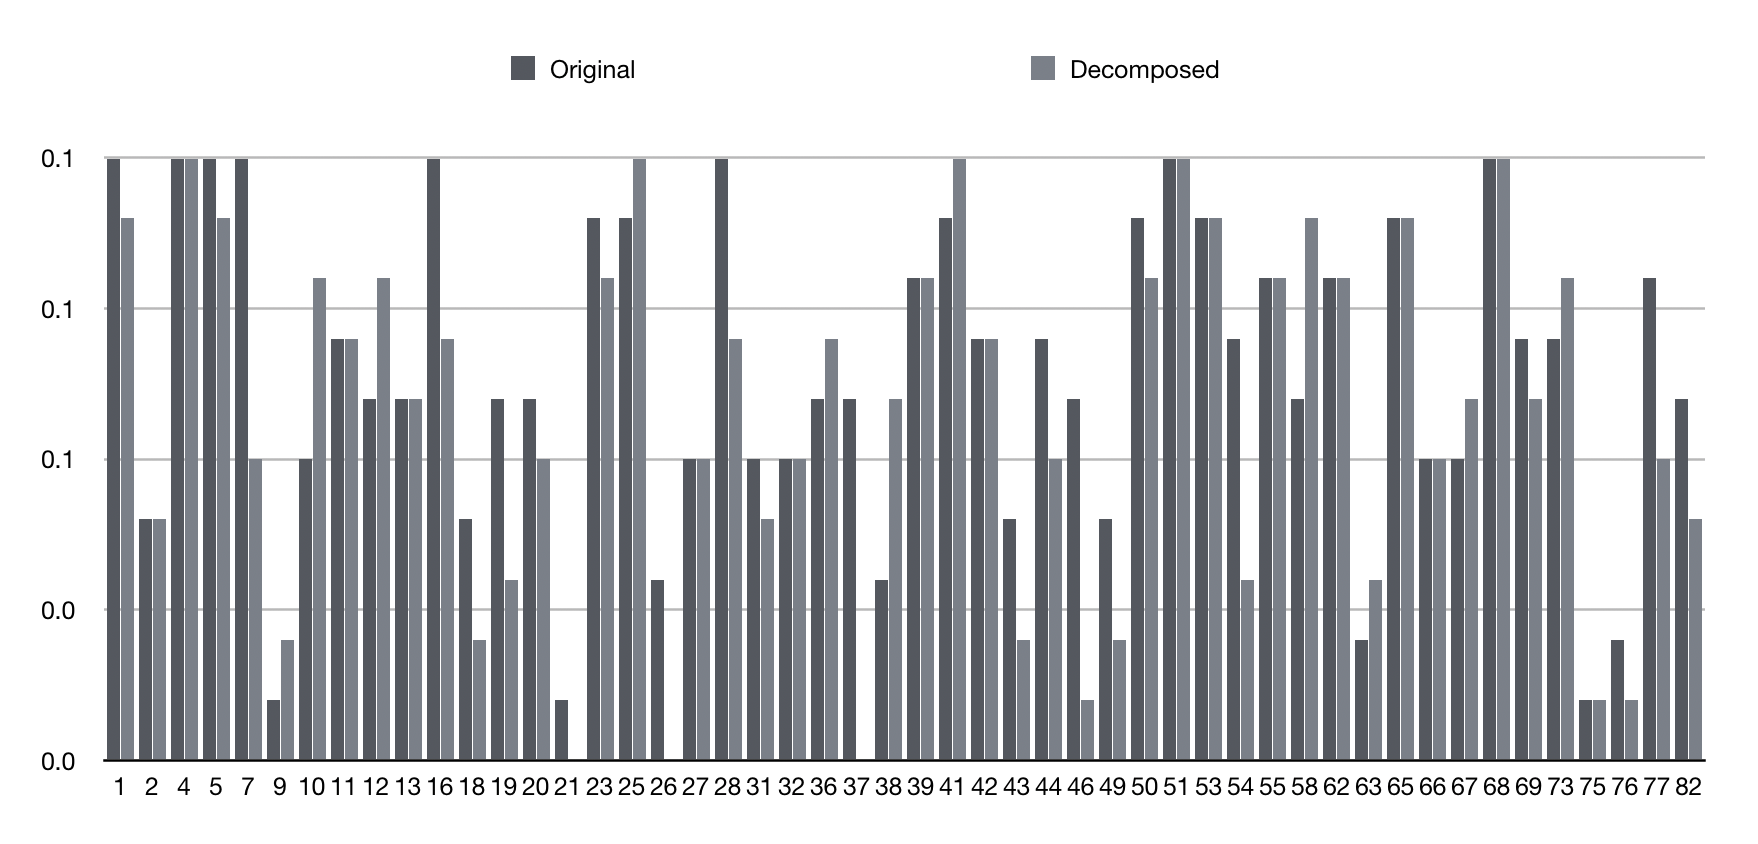
\includegraphics[width=1\textwidth]{p_at_10.png}
    \caption{P@10 Score for the Original and Decomposed Corpus}
\end{figure}

Some of the precision scores were higher in the original corpus, but there are still some that were higher in the decomposed corpus. In general, those whose title contain compounds are more likely to gain from the decomposed corpus, such as topic 10 ``Att behandla med xenical vid samtidig diabetes och/eller högt blodtryck''. ``blodtryck'' is a compound means ``blood pressure'' in English so it makes sense that doing a query with \verb|#combine(bold tryck)| should match more articles.

\begin{table}[h]
    \begin{center}
        \begin{tabular}{c|c|c|}
            \textbf{K} & \textbf{Precision Origianl} & \textbf{Precision Decomposed} \\
            \hline
            1  & 0 & 1 \\
            2  & 0.5 & 1 \\
            3  & 0.333 & 0.667 \\
            4  & 0.5 & 0.75 \\
            5  & 0.6 & 0.6 \\
            6  & 0.667 & 0.67 \\
            7  & 0.714 & 0.571 \\
            8  & 0.75 & 0.5 \\
            9  & 0.667 & 0.444 \\
            10  & 0.6 & 0.4 \\
            20  & 0.5 & 0.5 \\
            30  & 0.367 & 0.5 \\
            50  & 0.320 & 0.52 \\
            100  & 0.220 & 0.41 \\
        \end{tabular}
        \label{tab_k_value}
        \caption{Precision Scores for Topic 82 at Different $K$}
    \end{center}
\end{table}

Table \ref{tab_k_value} shows the effect of different K values on Topic 82. As we see in the original corpus, the higher the k is the higher the precision score is, until $k=8$. This is reasonable since there should be more relevant articles as our result set grows. However things changed a little bit in the decomposed corpus. There the highest score happens when k was in a very small value, then it decreases to 0.4 before climbing up again.

So it looks like the best k value depends both on the topic and the corpus. Nevertheless, setting $k$ at a big value isn't the best strategy to get a high precision score.

\section{MAP}
The MAP score on the decomposed compound set is slightly worse at 0.402, about 0.04 lower than the one on the regular document set. This can be attributed to the fact that the titles from the topic file were not decomposed, plus the \verb|#combine()| operator matches the whole word for compound words instead of their components.

\end{document}